\chapter{Software}
\section{Campionamento}
\begin{figure}[H] \centering
    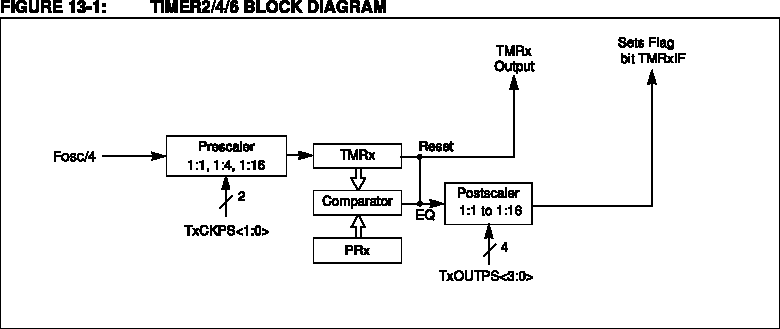
\includegraphics[width=.9\linewidth]{figures/timer2-block-diagram}
    \caption{
        Schema a blocchi del TIMER2. Fonte: Microchip PIC18F2X/4XK22 datasheet
        \label{fig:timer2-diagram}
    }
\end{figure}

\section{Trasferimento dei dati}
Per trasferire i dati campionati era inizialmente stato scelto di utilizzare
una struttura dati binaria. In seguito per\`o per 

\section{Interfaccia al Computer}
Per preferenze principalmente personali \`e stato scelto di realizzare
l'interfaccia al computer utilizzando il moderno linguaggio di programmazione
C++ (versione \(\geq\) 11) utilizzando un framework (Qt) che sar\`a descritto
successivamente.  I vantaggi dati dall'utilizzo del C++ anzich\`e linguaggi
interpretati come il Python, linguaggi compilati in bytecode come Java, o con
runtime particolari come LabView / CVI sono molteplici. Innanzitutto tutti gli
strumenti necessari per lo sviluppo hanno mezzi o varianti \emph{open source /
libre}, di conseguenza gratuiti e in molti casi multipiattaforma. Al contrario
invece dei sistemi proprietari come quelli offerti da National Instruments che
sono estremamente costosi e possono essere utilizzati unicamente sulle
piattaforme con un supporto ufficiale.  Tra i vari linguaggi di programmazione
non proprietari il C++ \`e comunque in posizione di vantaggio siccome \`e tra
i pi\`u performanti in quanto non richiede alcun interpreter (bytecode o non)
o nessuna runtime, stando quindi alla pari con il linguaggio C guadagnando
per\`o i vantaggi dell'astrazione data dalla programmazione ad oggetti.

\subsection{Librerie e codice di terzi}
Per ridurre i tempi dedicati alla realizzazione del programma, seppur
mantenendo una buona qualit\`a, \`e stato scelto di utilizzare le seguenti
librerie.

\begin{itemize}
    \item Serial (\url{http://wjwwood.io/serial/}): Utilizzata come
        interfaccia multipiattaforma per l'accesso di basso livello alla porta
        seriale del sistema operativo sottostatante. Descrizione dal sito:
        \begin{displayquote}
            This is a cross-platform library for interfacing with rs-232
            serial like ports written in C++. It provides a modern C++
            interface with a workflow designed to look and feel like PySerial,
            but with the speed and control provided by C++. 
        \end{displayquote}

    \item QCustomPlot (\url{http://qcustomplot.com}): Utilizzata per produrre
        il grafico all'interno del software, per visualizzare i dati dal
        microcontroller. Descrizione dal sito:
        \begin{displayquote}
            QCustomPlot is a Qt C++ widget for plotting and data
            visualization. It has no further dependencies and is well
            documented. This plotting library focuses on making good looking,
            publication quality 2D plots, graphs and charts, as well as
            offering high performance for realtime visualization applications. 
        \end{displayquote}
\end{itemize}

\subsection{Qt Framework}
La dipendenza principale utilizzata per realizzare la grafica \`e il framework
di Qt. Oggi Qt \`e un'azienda indipendente che vende un supporto commerciale
per lo sviluppo di applicazioni su praticamente ogni piattaforma.
Qt \`e un framework maturo che esiste oramai da 22 anni ed \`e disponibile sia
con una licenza commerciale che con le licenze open source LGPL e GPL.

La toolchain di Qt aggiunge al normale sviluppo un preprocessore speciale
chiamato MOC che genera in automatico il codice dalle strutture grafiche
realizzate con QtDesigner. Il resto della toolchain \`e composta da componenti
tipici che possono essere intercambiati liberamente poich\`e Qt supporta
gcc/g++, clang, MSVC e MinGW. Per compilare il codice \`e dunque necessario un
compiler qualsiasi di C++ e l'IDE QtCreator, oppure qmake. Poch\`e questi
pacchetti offrono il preprocessore MOC. Per progetti open source entrambi sono
offerti gratuitamente dal sito ufficiale \url{www.qt.io}.

\subsection{Compilazione sotto Linux}
Il programma \`e stato realizzato in parte sotto Debian 9.4 Stretch ed in
parte sotto Fedora 27. Per entrambi i sistemi sono necessarie le dipendenze
per lo sviluppo in Qt5.

\noindent Una volta installate le dipendenze dalla cartella di progetto \`e
possibile utilizzare il makefile per compilare le dipendenze e il codice.
\begin{Verbatim}[frame=single]
$ make build-deps   # dependencies
$ make              # spectrum analyzer code 
\end{Verbatim}
Purtroppo la liberia QCustomPlot utilizza un sistema di build molto
particolare che richiede molte dipendenze. Perci\`o in alcuni casi \`e
preferibile scaricare dal seguente link l'ultima versione dei due files
\texttt{qcustomplot.cpp} e \texttt{qcustomplot.hpp} ed immetterli manualmente
nella cartella \texttt{lib/qcustomplot/}.
\begin{center}
\url{http://qcustomplot.com/index.php/download}
\end{center}
Ed infine si compila con
\begin{Verbatim}[frame=single]
$ make serial       # build only Serial library dep
$ make              # build spectrum analyzer code 
\end{Verbatim}

\subsection{Compilazione manuale sotto Linux}
Per compilare manualmente il progetto sono necessari pochi steps grazie a
qmake. Come per il caso precedente la libreria QCustomPlot pu\`o essere
scaricata dal sito.

\begin{enumerate}
\item Scaricare le dipendenze.
\begin{Verbatim}[frame=single]
$ git submodule init
$ git submodule update
\end{Verbatim}

\item Compilare la libreria Serial
\begin{Verbatim}[frame=single]
$ mkdir -p lib/build-serial
$ qmake -makefile -o Makefile -Wall "CONFIG+=releae" \
    -o lib/build-serial/ lib/serial

$ make -C lib/build-serial/
\end{Verbatim}

\item Compilare la libreria QCustomPlot
\begin{Verbatim}[frame=single]
$ cd lib/qcustomplot/src
$ sed -i -e 's/qmake474/qmake/' release.py
$ ./release.py
$ cd ../.. # go back to project root dir
\end{Verbatim}

\item Compilare il progetto
\begin{Verbatim}[frame=single]
$ mkdir -p build-deskop
$ qmake -makefile -o Makefile -Wall "CONFIG+=release" \
    -o build-desktop/ src-desktop

$ make -C build-desktop
\end{Verbatim}
\end{enumerate}

\subsection{Compilazione sotto Windows}
Per compilare il progetto in Windows \`e necessario installare QtCreator dal
sito ufficiale \url{www.qt.io}.

\begin{enumerate}
\item Installare QtCreator, Qt \(\geq\) 5.0 (consigliato 5.10.0)
\item Installare MinGW oppure MSVC + Visual Studio (consigliato MinGW)
\item Inizializzare ed aggiornare i submoduli di Git oppure clonare
    recursivamente il progetto.
\item Scaricare dal sito \url{http://qcustomplot.com/index.php/download} i
    documenti \texttt{qcustomplot.cpp} \texttt{qcustomplot.hpp} della libreria
    QCustomPlots ed immetterli nella cartella \texttt{lib/qcustomplots/}
\item Aprire il progetto \texttt{lib/serial/serial.pro} ed impostare la
    build directory sia per release che per debug in \texttt{lib/build-serial}.
\item Compilare la libreria Serial come release.
\item Aprire il progetto \texttt{src-desktop/SpectrumAnalyzer.pro} ed
    impostare la cartella di build sia per release che debug nella cartella
        \texttt{build-desktop/}
\item Compilare il progetto SpectrumAnalyzer come release
\item Controllare che lo script \texttt{deploy-desktop.cmd} abbia le variabili
    \texttt{QT\_PATH} e \texttt{QT\_VERSION} che corrispondano con la vostra
    l'installazione.
\item Eseguire lo script \texttt{deploy-desktop.cmd}.
\end{enumerate}
Nella cartella \texttt{build-desktop} sar\`a pronto l'eseguibile con tutte le
librerie dinamiche (DLL) necessarie.

\subsection{Architettura}
Il programma desktop \`e programmato per agire ad eventi asincroni dati dalla
porta seriale del sistema operativo e dalle interazioni dell'utente.
La gestione degli eventi grafici \`e gestita interamente da Qt, perci\`o sono
stati scritti solamente i metodi che vengono attivati in funzione degli eventi
dall'utente.

Per la porta seriale invece il compito della gestione \`e stato delegato ad una
classe \texttt{SerialWorker} che ha un rapporto di \emph{composizione} con la
classe \texttt{MainWindow} in quanto essa esiste unicamente quando esiste
\texttt{MainWindow}. Nella figura \ref{fig:desktop-sequence} \`e mostrato un
diagramma delle sequenze che mostra il flusso dei dati attraverso le
componenti del programma.

\begin{figure}[H] \centering
    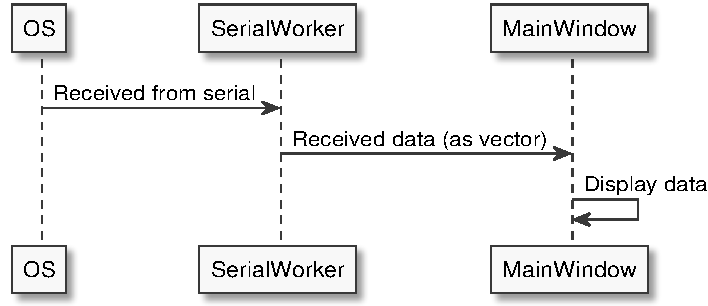
\includegraphics[width=.6\textwidth]{figures/uml/desktop-sequence}
    \caption{Diagramma delle sequenze \label{fig:desktop-sequence}}
\end{figure}

Per l'implementazione nella figura \ref{fig:desktop-classes} \`e possibile
osservare il diagramma UML delle classi. \`E importante notare che Qt 
introduce dei nuovi tipi di membri chiamati \emph{slots} e \emph{signals}.
Gli slots sono dei normali metodi che rispondo ai signals. I signals invece
sono delle funzioni prive di implementazione che possono essere \emph{emesse}.

Quando viene realizzato un modello ad oggetti in Qt \`e possibile collegare
degli slots a dei segnali per poter gestire delle azioni asincrone.  Nel
progetto dello SpectrumAnalyzer il segnale \texttt{receivedData} della classe
\texttt{SerialWorker} viene messo quando sono stati ricevuti dei dati validi
dalla seriale. Il segnale ha come argomento un vettore di numeri complessi
interi.

Nella classe \texttt{MainWindow} il segnale di \texttt{receivedData} \`e
associato allo slot \texttt{serialDataReceiver} con argomento uguale al
segnale, dunque un vettore di numeri complessi interi, che processa i dati e li
mostra nell'interfaccia utente.

\begin{figure}[H] \centering
    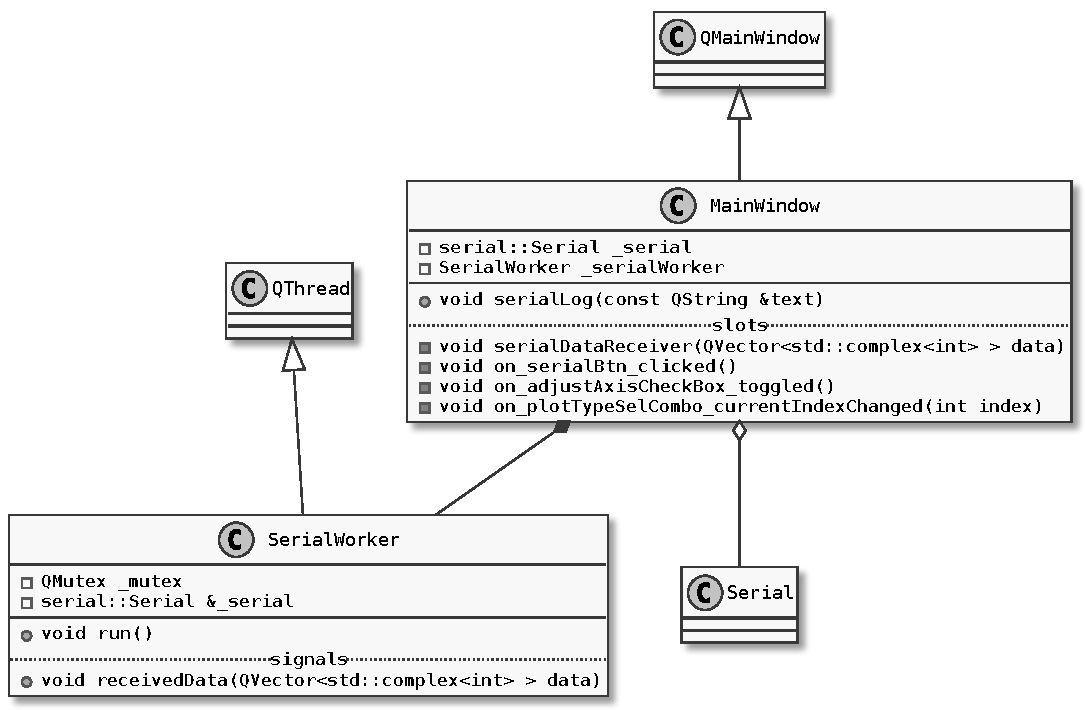
\includegraphics[width=\textwidth]{figures/uml/desktop-classes}
    \caption{Diagramma delle classi \label{fig:desktop-classes}}
\end{figure}

\subsection{Interfaccia utente}
\begin{figure}[H] \centering
	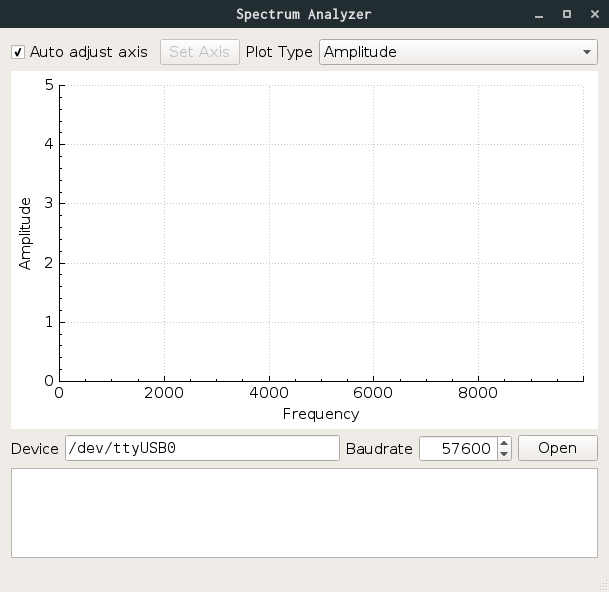
\includegraphics[width=.5\textwidth]{figures/screenshots/desktop-debian-empty}
\end{figure}

\section{Interfaccia al Display}

\section{Fast Fourier Transform}
